%++++++++++++++++++++++++++++++++++++++++
% Don't modify this section unless you know what you're doing!
\documentclass[UTF8,a4paper,12pt]{article}
\usepackage{ctex}
\usepackage{titlesec}%设置页眉页脚
\usepackage{tabularx} % extra features for tabular environment
\usepackage{amsmath}  % improve math presentation
\usepackage{graphicx} % takes care of graphic including machinery
\usepackage[margin=1in,letterpaper]{geometry} % decreases margins
\usepackage{cite} % takes care of citations
\usepackage[final]{hyperref} % adds hyper links inside the generated pdf file
\hypersetup{
	colorlinks=true,       % false: boxed links; true: colored links
	linkcolor=blue,        % color of internal links
	citecolor=blue,        % color of links to bibliography
	filecolor=magenta,     % color of file links
	urlcolor=blue         
}
%++++++++++++++++++++++++++++++++++++++++
\newpagestyle{newpagestyle}{
\sethead{\textit{现代物理实验}}{
\includegraphics[width=0.25in,height=0.25in]{zju}}{\textit{Physics Department}}
\headrule
}
\pagestyle{newpagestyle}

\begin{document}
\bibliographystyle{unsrt}
\title{\huge{激光的声光频移实验报告}}
%\author{黄敏 21636046}
\date{}
\maketitle

\thispagestyle{newpagestyle}


\begin{center}
\large{姓名:\underline{ 黄敏}}\hspace{1cm}
\large{学号:\underline{ 21636046}}\hspace{1cm}
\large{实验日期:\underline{ \textit{2017.3.21}}}
\end{center}
\section{实验目的}

\noindent 1.了解声光效应的原理,学习和掌握声光移频器的工作原理;\\
2.通过对声光器件衍射效率和带宽等的测量,加深对其概念的理解;\\
3.测量声光偏转和声光调制曲线。


\section{实验原理}
\subsection{声光效应的概念}
声光效应是光通过声波扰动的介质时发生散射或衍射的现象。
由于声波是一种弹性波,声波在介质中传播会产生弹性应力或应变,这种现象称为弹光效应。由于弹光效应,当超声纵波以行波形式在介质中传播时会使介质折射率产生正弦或余弦规律变化,出现疏密相间的现象,如同一个相位光栅。并随超声波一起传播,当激光通过此介质时,就会发生光的衍射,即声光衍射。衍射光的强度、频率、方向等都随着超声波场而变化。其中衍射光偏转角随超声波频率的变化而变化的现象称为声光偏转;衍射光强度随超声波功率的变化而变化的现象称为声光调制。
主要用途有:制作声光调制器件,声光偏转器件,声光调Q开关,可调谐滤光器,在光信号处理和集成光通讯方面也有应用。

%\begin{center}
%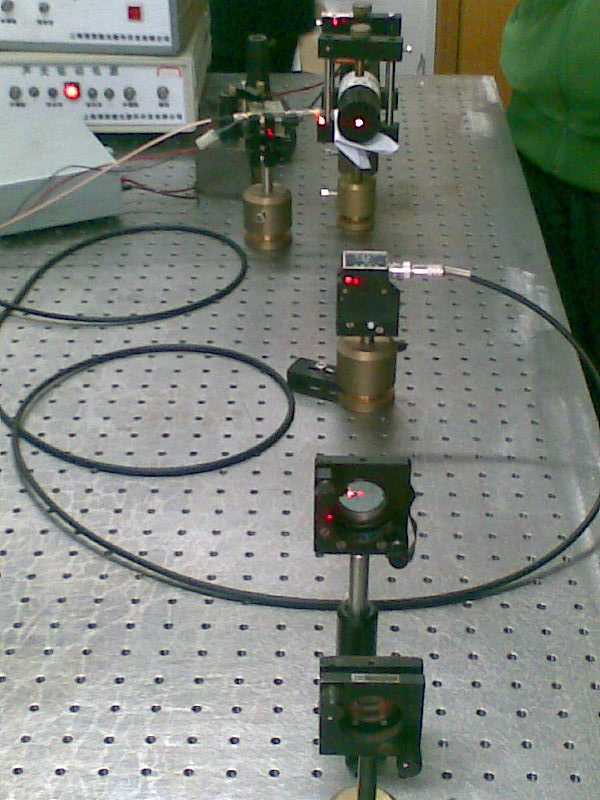
\includegraphics[width=10.5cm,height=10.5cm]{shiwutu}
%\end{center}


\subsection{声光效应的原理}
\subsubsection{布拉格衍射}
当超声波在介质中传播时,将引起介质的弹性应变作时间上和空间上的周期性的变化,并且导致介质的折射率也发生相应的变化。当光束通过有超声波的介质后就会产生衍射现象,这就是声光效应。有超声波传播的介质如同一个相位光栅。
\begin{figure}[htbp] 
 \begin{center} 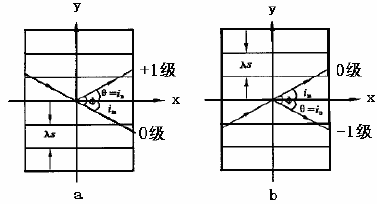
\includegraphics[width=8cm,height=6cm]{bragyspm} 
 \caption{\label{fig:bragyspm}布拉格衍射平面}
\end{center}
我们利用声光耦合波理论来分析布拉格衍射,考虑超声波和光波均为平面波且在各向同性介质中互作用的情况,各向同性介质中波动方程和受超声波调制的介质折射率$\vec{n}(\vec{r},t)$分别为:

\centering $\nabla^2\vec{E}(\vec{r},t) = \dfrac{{\vec{n}}^2(\vec{r},t)}{c^2}\dfrac{\partial^2\vec{E}(\vec{r},t)}{\partial t^2}$\\
 \centering $\vec{n}^2(\vec{r},t) = n+\Delta n\cdot sin(\omega_s t-\vec{k_s}\cdot \vec{r})$


\end{figure}
\subsubsection{声光偏转}
\subsubsection{声光移频器}
\begin{equation*}
\begin{split}
E &= E_1+E_2  \\
&= E_0\cdot Re\{exp[i(k_1z-\omega_1t+\varphi_1)]+exp[i(k_2z-\omega_2t+\varphi_2)]\} \\
&= E_0[cos(k_1z-\omega_1t+\varphi_1)+cos(k_2z-\omega_2t+\varphi_2)]\\
&= 2E_0cos[\dfrac{(k_1-k_2)z-(\omega_1-\omega_2)t+(\varphi_1-\varphi_2)}{2}]cos[\dfrac{(k_1+k_2)z-(\omega_1+\omega_2)t+(\varphi_1+\varphi_2)}{2}]
\end{split}
\end{equation*}
现在令$\Delta k=k_1-k_2,\Delta \omega=\omega_1-\omega_2,\Delta \varphi=\varphi_1-\varphi_2$,$k_0=\dfrac{k_1+k_2}{2},\omega_0=\dfrac{\omega_1+\omega_2}{2},\varphi_0=\dfrac{\varphi_1+\varphi_2}{2}$,则上式可以写成:
\begin{equation*}
E = 2E_0cos(\dfrac{\Delta k z-\Delta{\omega} t+\Delta \varphi}{2})cos(k_0 z-\omega_0 t+\varphi_0)
\end{equation*}


\section{实验主要步骤}
\begin{figure}[htbp] 
 \centering 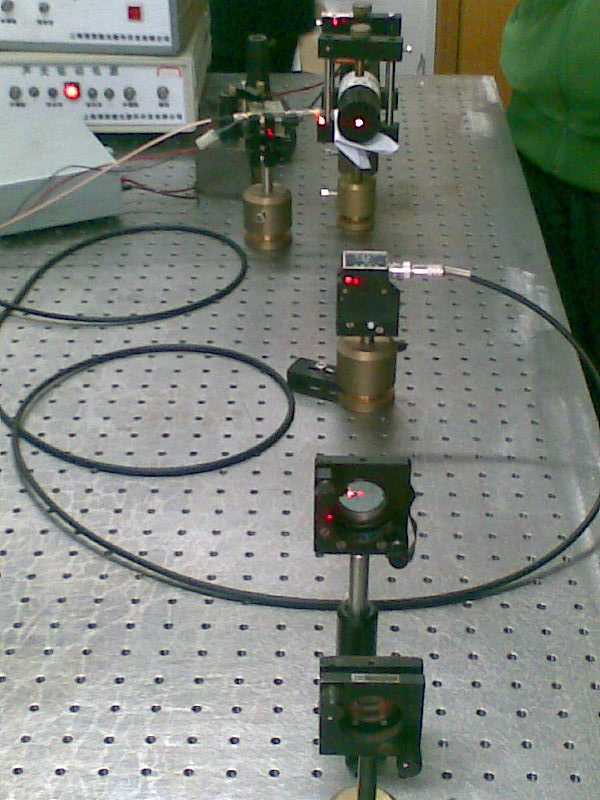
\includegraphics[width=8cm,height=10cm]{shiwutu}
 \caption{\label{fig:shiwutu}实验光路实物图}
\end{figure}
Give a schematic of the experimental setup(s) used in the experiment (see
figure~\ref{fig:samplesetup}). Give the description of  abbreviations
either in the figure caption or in the text. Write a description of what is
going on. 

\begin{figure}[ht] 
        % read manual to see what [ht] means and for other possible options
        \centering 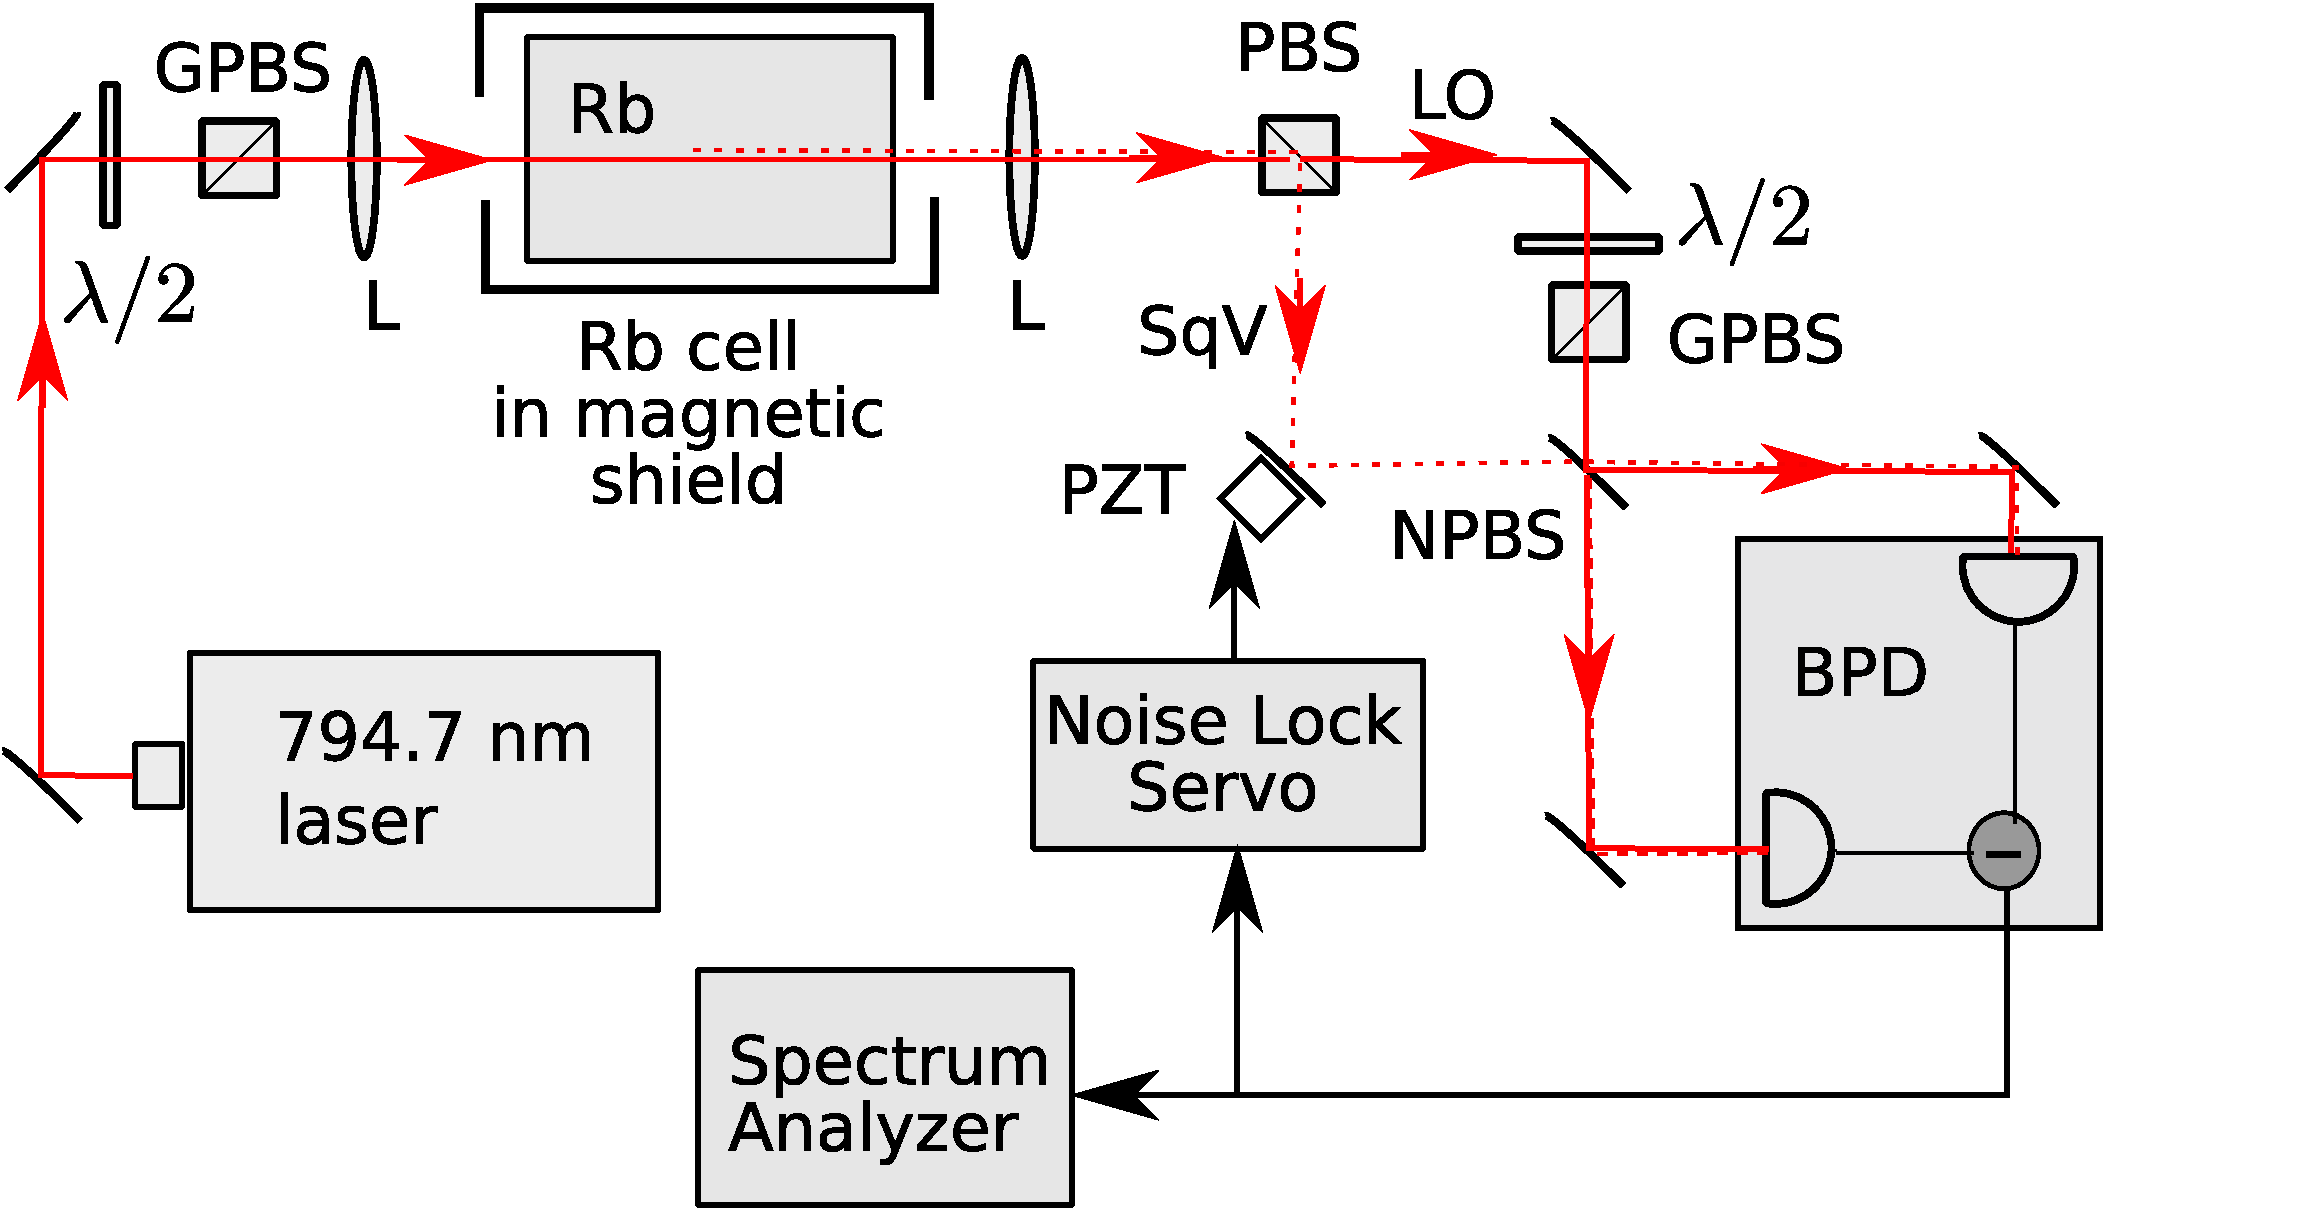
\includegraphics[width=0.8\columnwidth]{sr_setup}
        % note that in above figure file name, "sr_setup",
        % the file extension is missing. LaTeX is smart enough to find
        % apropriate one (i.e. pdf, png, etc.)
        % You can add this extention yourself as it seen below
        % both notations are correct but above has more flexibility
        %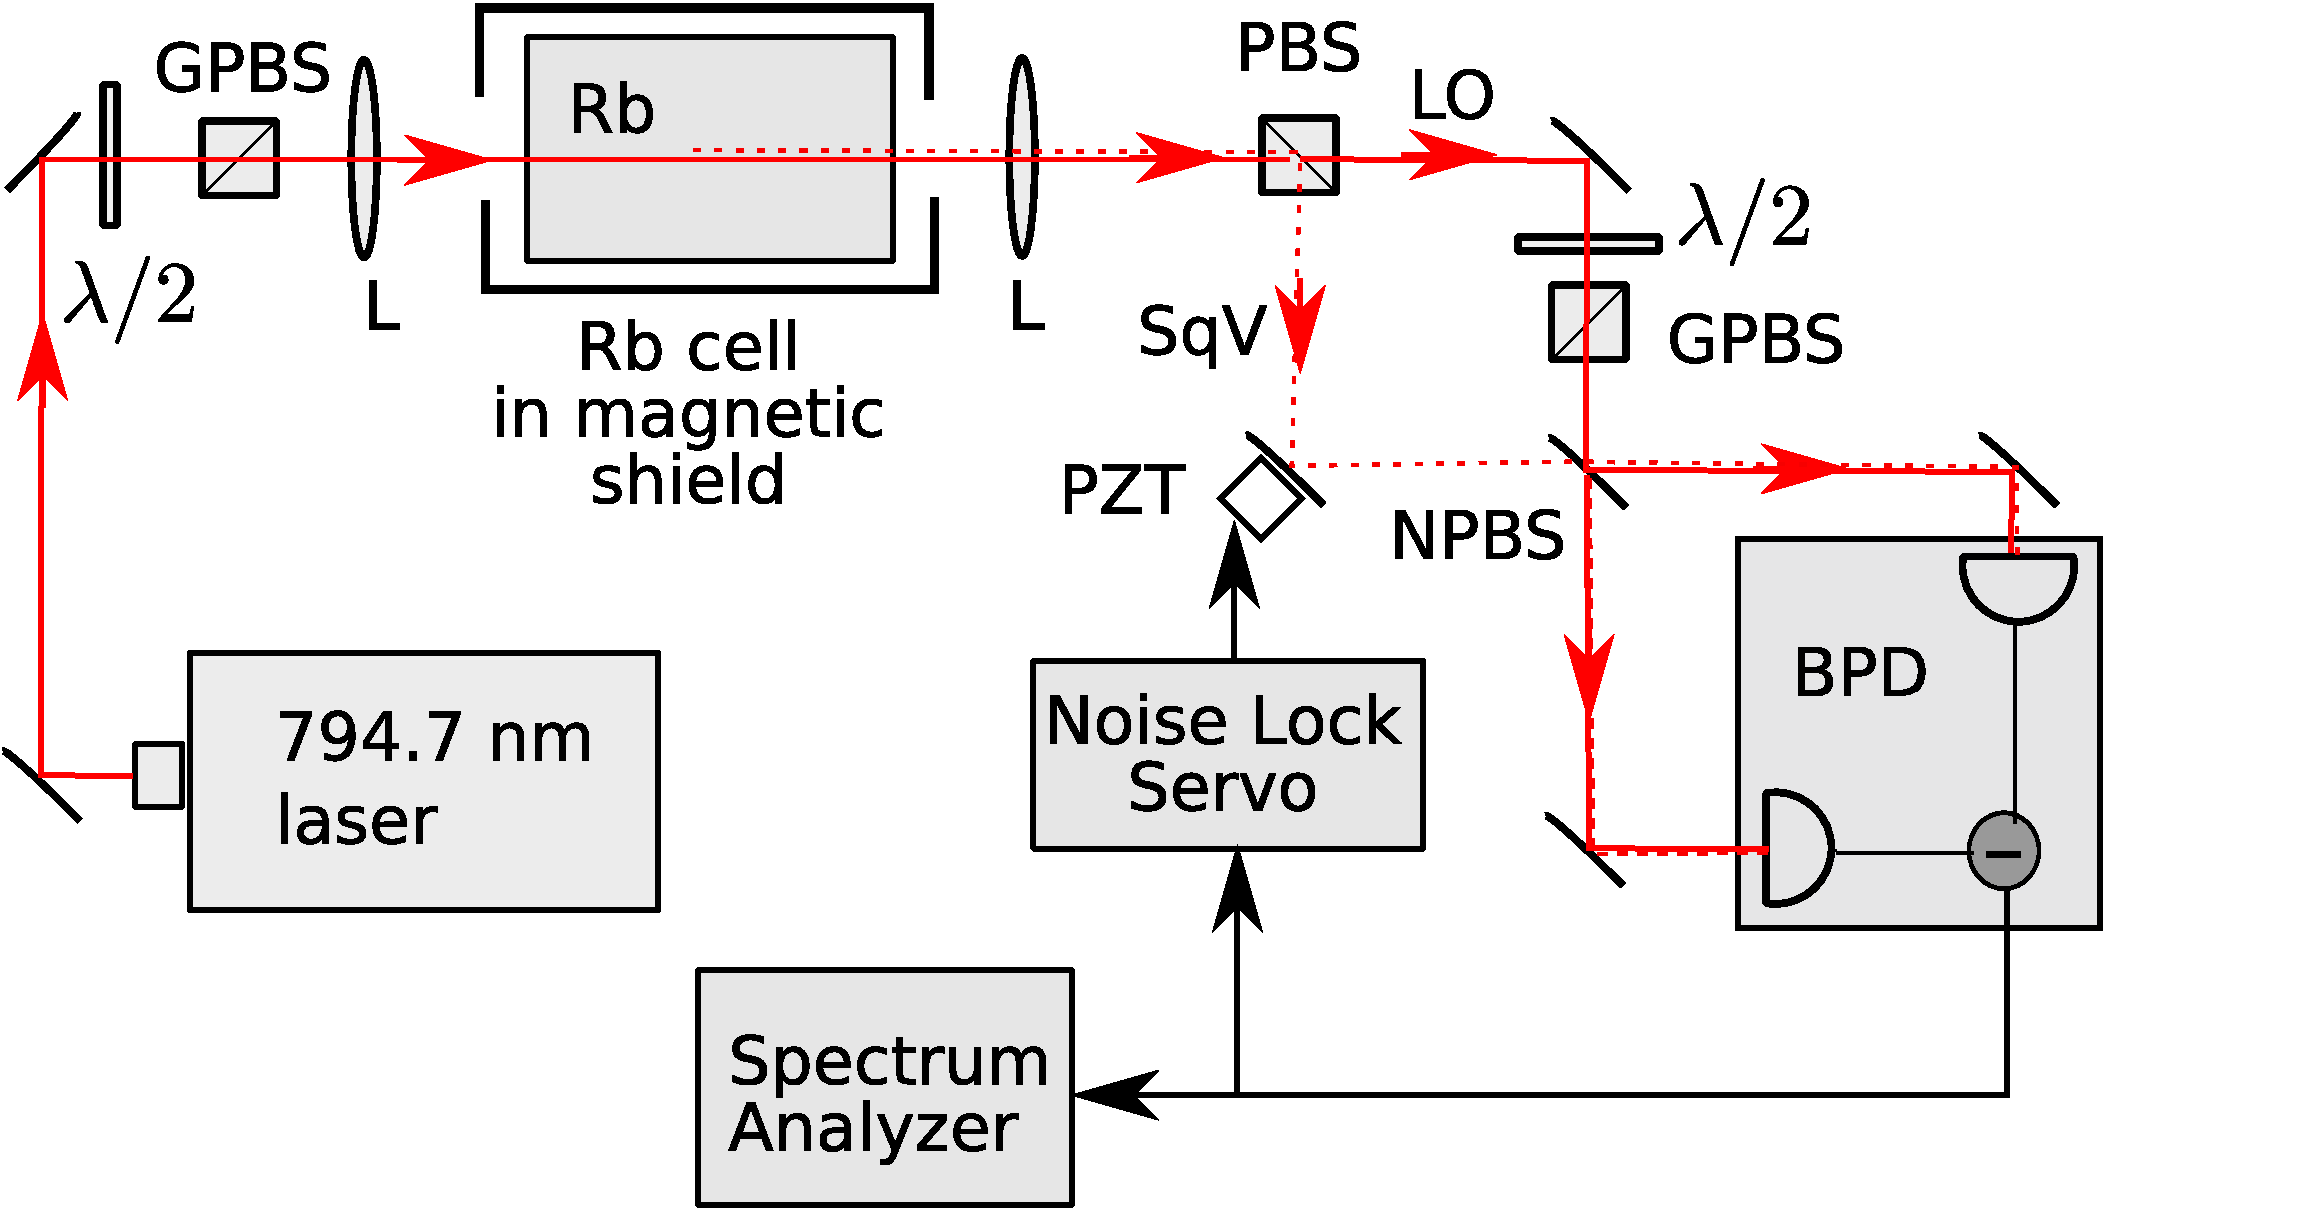
\includegraphics[width=1.0\columnwidth]{sr_setup.pdf}
        \caption{
                \label{fig:samplesetup} % spaces are big no-no withing labels
                % things like fig: are optional in the label but it helps
                % to orient yourself when you have multiple figures,
                % equations and tables
                Every figure MUST have a caption.
        }
\end{figure}

Don't forget to list all important steps in your experimental procedure!

Use active voice either in past or present through all the report and be
consistent with it:
The laser light comes  from to ... and eventually arrived to the
balanced photodiode as seen in the figure~\ref{fig:samplesetup}.

Sentences in the past voice while correct are generally considered hard to read
in large numbers. The laser light was directed to ..., wave plates were set
to ... etc.


\section{数据分析及实验结果}

In this section you will need to show your experimental results. Use tables and
graphs when it is possible. Table~\ref{tbl:bins} is an example.

\begin{table}[ht]
\begin{center}
\caption{Every table needs a caption.}
\label{tbl:bins} % spaces are big no-no withing labels
\begin{tabular}{|cc|} 
\hline
\multicolumn{1}{|c}{$x$ (m)} & \multicolumn{1}{c|}{$V$ (V)} \\
\hline
0.0044151 &   0.0030871 \\
0.0021633 &   0.0021343 \\
0.0003600 &   0.0018642 \\
0.0023831 &   0.0013287 \\
\hline
\end{tabular}
\end{center}
\end{table}

Analysis of equation~\ref{eq:aperp} shows ...

Note: this section can be integrated with the previous one as long as you
address the issue. Here explain how you determine uncertainties for different
measured values. Suppose that in the experiment you make a series of
measurements of a resistance of the wire $R$ for different applied voltages
$V$, then you calculate the temperature from the resistance using a known
equation and make a plot  temperature vs. voltage squared. Again suppose that
this dependence is expected to be linear%~\cite{Cyr}
, and the proportionality coefficient
is extracted from the graph. Then what you need to explain is that for the
resistance and the voltage the uncertainties are instrumental (since each
measurements in done only once), and they are $\dots$. Then give an equation
for calculating the uncertainty of the temperature from the resistance
uncertainty. Finally explain how the uncertainty of the slop of the graph was
found (computer fitting, graphical\cite{kiker2006qnd} method, \emph{etc}.)

If in the process\cite{chen}of data analysis you found any noticeable systematic
	error(s), you have to explain them in this section of the report\cite{witthaut} .

It is also recommended to plot the data graphically to efficiently illustrate
any points of discussion. For example, it is easy to conclude that the
experiment and theory match each other rather well \cite{peil}if you look at
Fig.~\ref{fig:samplesetup} and Fig.~\ref{fig:exp_plots}.

\begin{figure}[ht] 
  \centering
      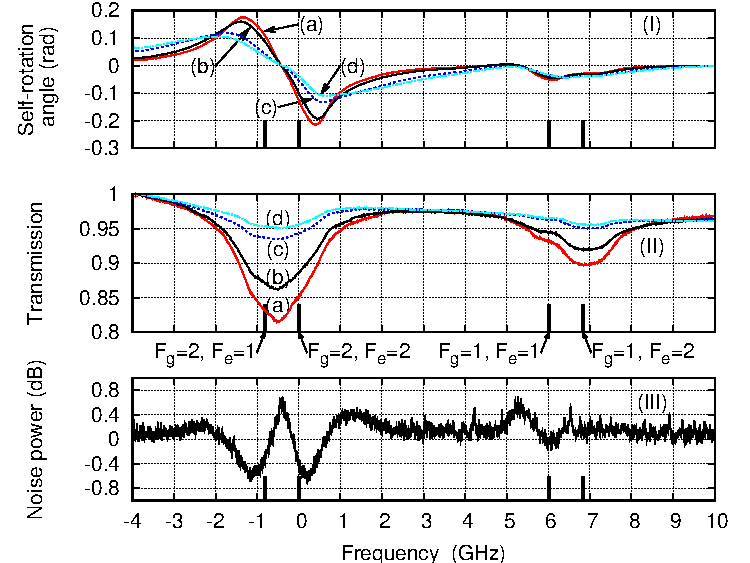
\includegraphics[width=0.5\columnwidth]{sr_squeezing_vs_detuning}

% some figures do not need to be too wide
        \caption{
                \label{fig:exp_plots}  
                Every plot must have axes labeled.
        }
\end{figure}


\section{实验小结}
Here you briefly summarize your findings.

%++++++++++++++++++++++++++++++++++++++++
% References section will be created automatically 
% with inclusion of "thebibliography" environment
% as it shown below. See text starting with line
% \begin{thebibliography}{99}
% Note: with this approach it is YOUR responsibility to put them in order
% of appearance.

%\begin{thebibliography}{ABC}
%\bibitem{melissinos}
%A.~C. Melissinos and J. Napolitano, \textit{Experiments in Modern Physics},
%(Academic Press, New York, 2003).

%\bibitem{Cyr}
%N.\ Cyr, M.\ T$\hat{e}$tu, and M.\ Breton,
 %"All-optical microwave frequency standard: a proposal,"
%IEEE Trans.\ Instrum.\ Meas.\ \textbf{42}, 640 (1993).

%\bibitem{Wiki} \emph{Expected value},  available at
%\texttt{http://en.wikipedia.org/wiki/Expected\_value}.


%\end{thebibliography}

\bibliography{ref}


\end{document}
